\documentclass{mpaper}

\usepackage[colorinlistoftodos]{todonotes}
\usepackage{listings}
\usepackage[newfloat]{minted}
\usemintedstyle{emacs}
\usepackage{enumerate}
\usepackage{enumitem}
\usepackage{algorithm2e}

\newcommand{\code}[1]{\texttt{#1}}
\newenvironment{codelisting}{\captionsetup{type=listing}}{}
\SetupFloatingEnvironment{listing}{name=Code Sample}

% Use “\cite{NEEDED}” to get Wikipedia-style “citation needed” in document
\usepackage{ifthen}
\let\oldcite=\cite
\renewcommand\cite[1]{\ifthenelse{\equal{#1}{NEEDED}}{\ensuremath{^\texttt{[citation~needed]}}}{\oldcite{#1}}}

\newcommand{\remove}[1]{\textcolor{red}{#1}}

\begin{document}

\title{Smart Sensitivity Review}
\author{Kelvin Fowler}
\matricnum{2083905f}

\maketitle
\small{Note: Joint Honours - 40 Credits}
\remove{Tone down emphasis on sensitivity review}
\begin{abstract}
% Intro to Problem
Before documents are released to the public they must be reviewed for sensitivities. If a document's contents are already in the public domain then this document can be released to the public without going through the rigorous sensitivity review process.
Cross checking document contents with public domain documents is currently undertaken manually in an insecure and cumbersome way, involving users entering manual queries into public web search engines.
An automatic system could feasibly formulate queries from documents and retrieve public domain documents for cross referencing.
This query formulation from an arbitrary document is a difficult task, as these documents are potentially very long and contain much information.
We propose to use the extraction of named entities and temporal entities as key features in an automatic query generation.
We then use these terms in a complex query with a learning to rank strategy to learn which sections of this query are the most important for this task.
We evaluated this approach using a proxy test collection representative of the type of documents encountered in this task and found that our features show promise 

\remove{\textbf{conclude}}
% Why is it challenging
% how do you propose to address (why should it work)
% how evaluated
% what find
% conclusions
\end{abstract}

\section{Introduction} \label{sec:intro}
% Mention TNA in this first paragraph, understand the task, why are TNA even involved
Government departments have a responsibility to prevent sensitive information from being released to the public. Fortunately, some information in government documents already exists in the public domain. If a document contains only that information which is already in the public domain then it may skip the rigorous sensitivity review process.

Sensitivity review is a task carried out by government departments in the process of preparing documents for release to the general public. 
These documents are often requested as a result of the Freedom of Information Act, 2000~\footnote{\url{http://www.legislation.gov.uk/ukpga/2000/36}}. 
If a document is deemed to contain sensitive information then it may be withheld or redacted (this can also occur for other reasons)~\footnote{\url{https://ico.org.uk/for-organisations/guide-to-freedom-of-information/refusing-a-request/}}.
% Here you appear to say the same thing twice.
There are many reasons a document maybe be deemed sensitive\footnote{\url{http://www.legislation.gov.uk/ukpga/2000/36/part/II}}, however some examples are documents containing information which could negatively affect international relations or documents containing information which could put members of the armed or security forces at risk.

Part of this process involves cross checking document content with public domain information, as sensitive information which is already available to the public can be deemed not sensitive. 
Increasingly the documents which require review are digital and these documents are being generated at an ever increasing rate due to new technologies~\cite{allan2014record}. 
\remove{The National Archives also must decide which documents are worth keeping which in itself poses an interesting problem~\cite{moss2012have}, demonstrating further the scale of the these document collections.}


%Insert an example -- table format?
\begin{table*}[t]
\centering
\begin{tabular}{|p{8cm}|p{6cm}|}
\hline
Document Text & Potential Manual Query \\ \hline
This is an example document blah blah blah blah blah blah
& 1988 pubjab attack sikh gunmen khari sari
\\ \hline
\end{tabular}
\caption{An Example of manually forming a query to retrieve public domain documents}
\end{table*}

As a result, the current system of review must be improved to assist with this task as much as possible. Currently, the task of public domain comparison is undertaken by archivists manually searching for related public domain documents using web search engines.  This is a tedious task and exposes potentially sensitive information to external services.

This task lends itself well to the Information Retrieval (IR) space, since we must retrieve relevant public domain documents given a government record which is under consideration. 
IR tasks are usually carried out by issuing a query to a system.
% If this is a finding from last year cite, otherwise woolly claim
\remove{Of course,} it is not feasible to enter an entire document as a query, so we must consider which parts of the document are most important for the discovery of relevant public domain documents~\cite{DissertationKelvinFowler}.
By automating this process we reduce the risk of exposing sensitive information to outside services and also ease the task of the reviewer by forming queries and retrieving documents before the document is even manually read.

In this paper we describe techniques for document analysis which produce these queries when given a potentially sensitive document and issue them to a set of public domain documents. 
We mainly focus on named entities (people, places and organisations) and temporal entities (specific references in text to dates).
With these features extracted we combine them into complex query formulations.
Further we employ learning to rank techniques to automatically learn which aspects of these complex queries are the most important in the retrieval of relevant public domain documents.
These techniques are evaluated using a proxy test collection generated from an existing TREC test collection~\footnote{\url{https://trec.nist.gov/}}. This proxy collection was used for the purposes of learning models and experimentation, however some final experiments verified our approach upon a more representative test collection of WikiLeaks documents.

It should be noted that the goal of this paper is to provide a retrieval technique which can assist the manual process of public domain comparison in sensitivity review.
We do not seek to replace the manual aspect of this task and in fact archivists have made clear that they would be reluctant to trust technology alone~\cite{gollins2014using}.

% Defining Terminology
Throughout this paper we will refer to documents which are being reviewed as \textbf{source documents} and public domain documents which are being retrieved as \textbf{target documents.} Thus, queries will be formed from \textbf{source documents}.

% Research Questions from Proposal -- do we refer to proposal at all?

% We do/show that -- active verbs in contributions
% Make these precise
Our contributions are thus:
\begin{itemize}
\item We use a  new method for using complex query operators and learning to rank to implicitly learn the most important sections of queries.
\item \remove{We perform these complex queries and learning tasks in a new prototype version of Terrier.}
\item We generate a proxy test collection using existing relevance judgements in order to obtain data for learning an effective model.
\item We use temporal entities as an effective weak feature in the reranking of public domain documents. % by how much, do we even show this!
\item We contribute to the ongoing research surrounding the improvement of document review in government with an improved system for the ranking of public domain documents in the public domain comparison task.
\end{itemize}

The remainder of the paper will be structured as follows.
In Section~\ref{sec:background} we discuss the background of the project including related literature and limitations.
In Section~\ref{sec:complexquery} we explain the use of complex query formulations and operators in our research.
Section~\ref{sec:l2r} provides insight into our techniques for learning to rank, including what we deem to be interesting and potentially advantageous features.
Details on our experimental set-up are given in Section~\ref{sec:setup}, with our experimental results following in Section~\ref{sec:results}.
Finally, we conclude with discussion and avenues for future work in Section~\ref{sec:conclusion}.

\section{Background} \label{sec:background}
This section will discuss related literature to this research. We will discuss other approaches to sensitivity review and technology assited review. Temporal entities and their existing uses will be covered, as well as complex query formulations and learning to rank approaches. We will explain why this task cannot be completed to a sufficient standard at the moment with the discussed existing techniques and identify specifically what we aim to address.

\subsection{Sensitivity and Other Review}
% No background discussion of the use of named entities in IR
Applying information retrieval to assist sensitivity review is an ongoing problem and there are several potential avenues which have been attempted. 
Namely, the use of automatic classification of sensitivities can be seen in work by McDonald et al~\cite{mcdonald2014towards} through analysis of document sentiment and other features. More recently McDonald et al have attempted to include active learning in the sensitivity review process~\cite{mcdonald2018active}.

% TECHNOLOGY ASSISTED REVIEW -- EDISCOVERY/ CLINTON EMAILS/ TRY TO FIND A FRESH NEW EXAMPLE
More broadly, assisted sensitivity review comes under the banner of technology assisted review. This is mainly used in the realm of E-Discovery where opposing legal parties attempt to uncover as much information about each other as is possible. ~\cite{oard2013information}. This task seeks to obtain maximum recall (the retrieval of all relevant documents) so that neither party misses any details. In our case we are more concerned with precision in that archivists are unlikely to read all related documents during sensitivity review.

% Govt - http://www.nationalarchives.gov.uk/documents/technology-assisted-review-to-born-digital-records-transfer.pdf

% Clinton Emails -- speed of review.
In fact, this type of technology assisted review is becoming increasingly prevalent, featuring in news articles surrounding the 2016 U.S. Presidential Election~\footnote{\url{https://www.nytimes.com/2016/11/08/us/politics/hillary-clinton-donald-trump-fbi-emails.html}}. Technology allowed the F.B.I. to review 650,000 emails in a week through automatic classification and duplicate deletion.

% 4th YEAR PROJECT
This problem was tackled in part by a 4th year project at the University of Glasgow by us~\cite{DissertationKelvinFowler}. This lays the ground work for the more advanced research described in this paper. 
Our previous method relied on the use of named entities extracted from source documents in order to generate queries. The intuition was much the same as we described in Section~\ref{sec:intro}. There were, however, some key limitation in this work. Firstly, we extracted and tagged named entities only in a uni-gram manner. For example, given a document containing the name, ``Allen Hatcher'' the tokens \code{person\_allen} and \code{person\_hatcher} were produced. As such, we do not encode in queries that we seek documents only where ``Allen Hatcher'' is mentioned and not any other ``Allen'' or ``Hatcher''.
The results of \cite{DissertationKelvinFowler} showed that the full source documents (stopped and stemmed) could be used as a query however this was too slow for practical use. Slightly less performant but far faster was the use of all named entities as a query. Taking the top 10 named entities through Tf-Idf analysis was also attempted. Using the subject line of the document as query was also attempted.
This project also focussed on a UI for this assisted sensitivity review, which could be used in The National Archives.

Identified as missing were attempts to factor temporal information in documents into the queries. 
When dealing with sensitivities it is often important to consider the times of events. For example public domain articles about George Bush could refer to either Father or Son depending on the time period.

\subsection{Time in Information Retrieval}
As mentioned, time can be an important factor to consider in information retrieval, dependent on the task at hand. There are several technologies available for identification and resolution of temporal entities in documents such as Heideltime~\cite{strotgen2010heideltime} and SUTime~\cite{chang2012sutime}. These allows temporal expressions to be represented in a normalised format ideal for further manipulation and matching.

Str{\"o}tgen et al~\cite{strotgen2012identification} divide queries into a temporal part and textual part and examine how best to identify the most relevant temporal expressions in a document, both in general and with respect to a query. Of features they identify, value frequency is particularly relevant to us and we use this method for the comparison of the temporal aspects of source and target documents.

Jatowt et al~\cite{jatowt2013estimating} describe a method for approximating the focus time of a given document, however this requires connection to a knowledge base which is beyond the scope of this project. It is, however an interesting concept which we take some inspiration from in our attempts to make use of temporal entities in documents.

\subsection{Complex Queries}
% What are they.
Complex queries are IR queries which contain additional information than the plain text of regular queries. When producing a query from a large quantity of text it is useful to have these additional features as they can narrow a verbose query to be more targeted.

Terrier~\cite{macdonald2012puppy} implements parts of the Indri Query Language~\cite{strohman2005indri} which defines some of these complex query operators. Examples of complex query operators can be seen in Table~\cite{NEEDED}.

Lee et al~\cite{GeneratingQueriesLee12} use complex query operators in order to create queries from large arbitrary sections of text. Specifically Lee et al use these operators in order to weight sections of text they have extracted from the selected text. This has inspired our approach however we aim to apply the weighting through a learning to rank strategy, rather than a manual assignment.

\subsection{Learning to Rank}
% Introduction - properly explain what learning to rank is from scratch
Learning to rank (L2R) is a well used technique in information retrieval. It is a machine learning technique which learns how to rank documents in retrieval results in response to features and existing relevance data.
Learning to rank takes a sample of documents retrieved using some initial step and then re-ranks these documents based on features calculated.

Dang et al~\cite{dang2013two} discuss the sampling step of learning to rank, where we seek to retrieve as many relevant documents as possible (high recall) so that the second, learned reranking step can move as many relevant documents to high ranks as possible. Using this intuition we investigate which sampling set is the most effective.

% give an example of learning to rank which uses similar features to you

\subsection{Limitations of Existing Approaches} \label{sec:limitations}
% Here are all the limitations
\begin{enumerate}[label=\textbf{Limitation.\arabic*}, wide=\parindent]
\item To our knowledge the only previous attempt at assisting the public domain knowledge section of sensitivity retrieval was in our previous work in the L4 Project~\cite{DissertationKelvinFowler}. Thus, there is lack of information in the literature regarding this process.
\item The previous project did not seek to use temporal information to assist retrieval, while the literature clearly suggests that this could provide an improvement to performance. 
\item There is no clear gold standard test collection for this task, simply because it has not been attempted in previous literature.
\item Lee et al~\cite{GeneratingQueriesLee12} is perhaps the closest work to what we seek to achieve here, however their approach to generating queries from arbitrary sections of text is dependent on features which seek to find a general importance of concepts from the given text. They do not use learning to rank in order to allow the system to decide which features are most important.
\item In the previous project named entities were not represented in way which maintained multi-term relationships.
\end{enumerate}

\section{Overview of Approach}
% DIAGRAM
% Refer specifically to all of the limitations
In this section we present a high level overview of the approach we intend to take in order to tackle the limitations from Section~\ref{sec:limitations}, in order to ...

There is a lot of information in documents which could be used to form a query. It is not immediately obvious which parts of this information will produce the most effective query, as we have seen from the example in Table~\cite{NEEDED}. However, our approach involves the segmentation of queries into individual sections in order that a learning to rank strategy can determine which sections are most important for retrieval.

Creating these sectional queries means first extracting the key information from documents which we wish to turn into queries. We have seen that named entities are an intuitive choice from example and retrieval performance of named entity based queries from~\cite{DissertationKelvinFowler} reinforces this assumption.

Additionally, queries have a temporal component to them, in order to narrow search results to specific temporal window. In a similar way to the extraction of named entities, we can extract temporal entities from text. We will use this temporal information in our queries. \remove{NEED MORE REASONING}.

With these query components extracted, they must be formed into a comprehensive query which can be effectively passed to a learning to rank strategy.

With the introduction of Indri query language operators in Terrier 5, we are able to tag terms in queries as belonging to specific categories, among using other operations.

In learning to rank, we must define features. These features can must be scores that Terrier can calculate. Generally, pagerank might be used as a feature or another such score that we know about a document in response to query. Instead we define features which are only calculated on individual tagged sections of our query. See Table~\ref{table:features} for a list of the features we use in this research.

Figure~\ref{fig:approach} summarises our approach.
\begin{figure*}
\begin{center}
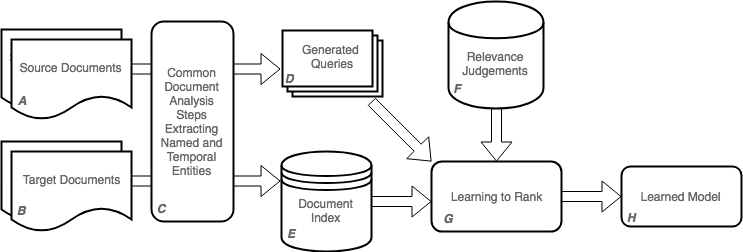
\includegraphics[scale=0.5]{5yp.png}
\end{center}
\caption{\label{fig:approach} The General Approach of Our System}
\end{figure*}


% List and refer back to the limitations
\section{Query Components}
In this section we describe the components that we extact from documents in order to formulate queries, including our use of named and temporal entities.
\begin{table*}[t]
\centering
\begin{tabular}{|p{8cm}|p{2cm}|p{2cm}|p{2cm}|}
\hline
Document Text & Named Entities  & Temporal Entities & Focus Times  \\ \hline
\textbf{Dukakis Loses Appeal Challenging Federal Authority Over National
Guard}

   A federal appeals court has rejected \textbf{Democratic} presidential candidate \textbf{Michael Dukakis'} attempt to use his power as governor to block a \textbf{Massachusetts} National Guard training mission in \textbf{Central America}.
   The \textbf{1st U.S. Circuit Court of Appeals} issued a one-sentence order \textbf{Tuesday} affirming a May 6 decision by \textbf{U.S. District} Judge \textbf{Robert Keeton}, who upheld federal supremacy over the National Guard.
   ``Having examined the briefs of the parties ... and having had the benefit of oral argument, we affirm the judgement on the basis stated in the district court's well-reasoned opinion,'' the appeals court said.
   \textbf{Dukakis} sued in January to block the assignment of 13 public relations specialists in the \textbf{Massachusetts} Guard to \textbf{Honduras} and \textbf{Panama} for two weeks in \textbf{May} because of his opposition to \textbf{Reagan} administration policies in the region.
   In his presidential campaign, \textbf{Dukakis} has denounced the administration for its ``failed and illegal'' policy of supporting \textbf{Nicaraguan} rebels, and he said sending Guard troops to the region was an attempt to intimidate \textbf{Nicaragua}.
   \textbf{Dukakis}, who was campaigning \textbf{Tuesday} in \textbf{California} and \textbf{Colorado}, had no immediate comment on the appellate decision. A press aide, \textbf{Steven Crawford}, said the governor was disappointed that the court chose not to uphold the ``important principle'' of state authority. ...
& items
& items
& items
\\ \hline
\end{tabular}
\end{table*}
In any given source document there is a lot of information. There are named entities, temporal entities and many other terms which provide context for a reader.
In order to effectively retrieve public domain documents we must decide which information is necessary to create a query. 
This section will describe in detail the methods used for extracting these items and the rationale behind our approaches.

\subsection{Named Entities}
% WHY DO WE EXTRACT THESE
% HOW DO WE EXTRACT THESE
% CAN WE DO ANYTHING EXTRA
In any given document, it is natural to seek to find out who the document is referring to. There is a notion that documents are often saying something about someone.
These ``someones'' can be called named entities. 
Methods exist for automatic extraction of named entities and the identification of which type of named entity is being used.
In this paper we will only consider named entities referring to persons, locations or organisations.
Named entities can be good indicators of who a document is speaking about.
Given a document about a bombing the mentions of ``ISIS'' and ``Syria'' can differentiate this document from other bombing elsewhere.
This intuition has encouraged us to use the extraction of named entities to improve query formulations.

These named entities occur in specific locations in the text, we can keep track of their positions and use this to formulate complex queries.

There is additional analysis we can perform on named entities.
A good indicator of a named entities importance, for example, may be it's Tf-Idf score in the collection of source document.

\subsection{Temporal Entities}
% WHY DO WE EXTRACT THESE
% HOW DO WE EXTRACT THESE
% CAN WE DO ANYTHING EXTRA
Temporal entities were resolved using the Heideltime temporal tagger. This allows us to identify temporal entities in text such as ``last Thursday'' and resolve this reference the specific date in question. To do this we must know the document creation date.
It is a reasonable assumption that these specific times are not of great use in and of themselves, since they are so numerous and so granular that matching on them will not produce any interesting behaviour. We confirm this with results in Section~\ref{sec:results}. As such it seems that it would be helpful to perform some analysis on the temporal entities which occur in a document.

We have opted for two approaches of calculating the focus time of a given document which contains temporal entities.
The first, median focus time $FT_{med}$, simply sorts the temporal references in a document and takes the median, assuming this to be some indication of the time which a document refers to.

The second method uses value frequency in order to calculate a focus time. These temporal entities which we resolve from text can come in various granularities. For example a document may contain the temporal entities seen in the example in Table~\ref{table:focustimes}.
% Identification and Resolution

\begin{table*}[t] \label{table:focustimes}
\centering
\begin{tabular}{|c|c|}
\hline
Temporal Entity 	& TimeX3 Representation  			\\ \hline
Last Thursday 		& <TIMEX3 12/04/18>Last Thursday</TIMEX3> 		\\ \hline
\end{tabular}
\caption{Examples of Resolved Temporal Entities and Subsequent Calculated Focus Times}
\end{table*}

% WHY DO WE EXTRACT THESE
% HOW DO WE EXTRACT THESE
% CAN WE DO ANYTHING EXTRA
In order to make use of the resolution of times in documents we opted to attempt to approximate focus times in documents. The intuition was that a target document was likely to be relevant in our task to a source document if they referred to similar times.
Direct matching of temporal entities was unlikely to be successful since even to adjacent days resolve to different tokens, and we have no concrete way of partial matching of terms.
Instead we devised several methods for the approximation of a documents focus time.
\textbf{Median Focus Time} - in order to calculate the median focus time all temporal references in a document are converted to their epoch offset equivalent (milliseconds from Jan. 1st 1970).
This collection was then sorted and the median date was taken to be the focus time.
This focus time was used to create three terms, a focus day, month and year. This allows for different granularities of matching.
Our approach is based on the intuition that if two documents produce median times of 16 June 1988 and 29th June 1999, then the fact that they both refer to June 1988 is still a good indicator of relevance.

\textbf{Value Frequency} - moving away from medians calculations this approach was inspired by \cite{strotgen2012identification} which identifies value frequency of temporal entities as being a good indicator for their importance.
As such this method was used to produce an additional approximate ``focus time''.
The method was as follow:

For every temporal entity of day granularity, the number of references in the text to that date were counted and the specific day with the most references was stored as the focus day.
Next every temporal entity with month granularity was counted and the most frequently occurring month was used as the focus month.

Last the most frequently occurring year was tagged as the focus year.

\remove{Give an example of the production of these focus times from a number of time references. Could kill 2 birds with one stone and display an example of the Heideltime process also.}

These calculations also seek to give an indication of the most important temporal entities in the text also.
 
\subsection{Additional Terms}
% WHY DO WE EXTRACT THESE
We extract these because the provide valuable context.

% HOW DO WE EXTRACT THESE
They are the terms which are left over.
We probably don't want to use them all.

% CAN WE DO ANYTHING EXTRA
We can calculate Tf-Idf scores on these terms to tell us how important they are.

\section{Learning with Complex Queries}
% WHY

% HOW

% ANYTHING ELSE INTERESTING

\section{Complex Query Formulations} \label{sec:l2r}
% Why do we want to use complex queries at all - for partitioning of the query into its component parts.
Queries can be composed of several labelled sections which denote meaning and content. 
Further, queries can contain complex operators which allow the user or system to issue rules which a information retrieval system must follow. For example, these might be that query terms must appear within a certain number of terms of each other.
Other uses are for describing synonyms (for example when someone searches for ``tea cup'' they may also receive results containing the term ``mug''.
These complex query formulations were used extensively in the experimentation of this system.

\begin{table*}[t] \label{table:features}
\centering
\begin{tabular}{|p{4cm}|p{6cm}|p{4cm}|}
\hline
Feature Name 		& Description  	& Representation \\ \hline
Person TF 			& TF Score for Person Named Entities 		& WMODEL\$person:Tf  \\ \hline
Location TF 		& TF Score for Location Named Entities 		& items  \\ \hline
Organisation TF 	& TF Score for Organisation Named Entities 		& items  \\ \hline
Time Terms Constant & Constant WM Matching on Temporal Terms			& items  \\ \hline
Vf Focus Year 		& Constant WM Matching on most frequently mentioned year. 		& items  \\ \hline
Vf Focus Month 		& Constant WM Matching on most frequently mentioned month (YY-MM).  		& items  \\ \hline
Vf Focus Day 		& Constant WM Matching on most frequently mentioned day (YY-MM-DD).  		& items  \\ \hline
Median Focus Year 	& pBiL 		& items  \\ \hline
Median Focus Month 	& pBiL 		& items  \\ \hline
Median Focus Day 	& Constant 		& items  \\ \hline
\end{tabular}
\end{table*}
Our approach is heavily centred around the subsequent use of learning to rank following the generation of complex queries.
Although we can generate these queries it is not immediately clear which sections of the queries are the most important for this public domain retrieval task.
As such, if we define our feature lists for learning to rank taking this partitioning into effect we can begin to understand what is important.
Learning to rank also allows the system to infer complex relationships between sections of queries that we may not understand.

\subsection{Sampling}
Since learning to rank is used to rerank the top k documents based on a certain set of features, it is optimal that this set of documents that is being reranked contains the highest possible number of relevant documents.
We aim to maximise recall at the initial stage of learning to rank so that upon reranking based on features we can promote as many relevant documents as possible.
\remove{refer to literature which talks about maximising the recall of sampling}

\textbf{Why cant we just retrieve all documents and calculate feature scores on every single one}
It is possible to achieve 100\% recall simply by retrieving all documents, however the calculation of feature scores across this amount of documents would take far too long for our needs. Why? Because we want fast retrieval~\cite{NEEDED} and people are only willing to wait so long on queries.

\subsection{Features}
The use of the Indri query language allowed us to define feature lists which used different retrieval models for individual sections of a query. For example we may have a feature which is the Tf score for only the person named entities in the text.

Named entities - why TF? There is data to support this~\cite{NEEDED}

term features
phrase features
proximity features
Use validation data to prevent over-fitting

LambdaMART - multiple additive regression trees, pointwise and listwise
NDCG is taken into account

\remove{need a diagram here explaining the method}

\section{Experimental Setup} \label{sec:setup}
This section will describe the steps taken to evaluate our system. We describe the test collections we use as well as the learning to rank configuration.

In the L4 Project~\cite{DissertationKelvinFowler} a small test collection was manually created. The topics were queries formed from 20 wikileaks documents, each of which had an associated 20 relevant public domain news articles. Because our approach in this research involves the use of learning to rank, we require a much larger collection of relevance judgements. It was not feasible create more manual relevance judgements as this would have been a very time consuming task.
Thus it was necessary to produce a test collection by some other means.

\remove{need some stronger evidence}
Having analysed the wikileaks collection of source documents it became clear that these documents generally followed a similar structure of reporting events from the viewpoint of various embassies. These reports exist to inform a reader about events happening at specific times, involving people, organisations and locations.

Now, news articles are very similar in nature to these wikileaks documents, as they also seek to report on events, the difference being that the content of a news articles is necessarily already in the public domain.
This similarity suggests that it may be possible to use news articles as representative source documents for the generation of queries.

Unfortunately, we did not have access to relevance judgements which defined news document as being relevant to one another.
Instead we chose to view the implicit relevance of documents to one another which are relevant for a common topic.

Given an existing TREC ad-hoc topic there exists a set of relevant public domain news articles. If two articles are relevant for the same topic, it suggests there is some information overlap in these documents.

Thus we made the assumption that if documents were relevant for the same topic then they were relevant to each other in our public domain comparison task.

The method described below for generating a test collection from existing topics and query relevance judgements are inspired by a method described by Lee et al~\cite{GeneratingQueriesLee12}.

In place of a full ground truth test collection we opted to generate a test collection from an existing ad-hoc TREC collection. This allowed us to avoid the lengthy and costly operation of obtaining results from volunteers.
The method to produce this test collection was as follows.

\remove{note that there is actually an additional topic set you could use for this 101-150, but we dont have time to go down this route}
Associated Press 1988 document corpus from TIPSTER disk 2.
TREC-1 ad hoc qrels (document set is TIPSTER disks 1\&2).
Our document set is only the AP88 set so if we remove all of the relevance judgements from other documents sets we reduce the numbers of qrels greatly.

Since we are only using AP88 as our test collection relevance judgements concerning any other documents were removed and ignored.

For each topic the corresponding relevance judgement were examined.
For a given topic T
If a document D was deemed relevant then a new qrels file was created.
For Q\_D (query made from document D), the following documents are deemed relevant.
All documents RD\\\{D\} which are relevant for the original topic T, with the document D removed so as to avoid self reference. A document can not be relevant for the query generated from itself. This caveat allowed us to avoid any additional complex indexing strategies.

\remove{which} Topic and Qrel set.

Our task is to produce inter document relevance.

When a document is relevant for a given topic, assume that if that document were a source document in our sensitivity review task, the the other documents which are relevant for that topic would be relevant target documents.

This test collection was generated from ... using the existing topics and qrels provided by TREC.
% Describe the use of the proxy test collection.

% Explain the algorithm, write on paper to get right first.
\begin{algorithm}
\SetAlgoLined
\KwResult{Proxy Test Collection}
 Get docs\;
 \For{t in T}{
  \For{doc in relevant docs}{
  add all other relevant docs to qrels\;
  \;
  }
 }
 \caption{Generating a Proxy Test Collection}
\end{algorithm}

\subsection{Learning to Rank}
In order to prevent over-fitting to training data during learning to rank we partitioned our test collection into training, validation and test sets.
This was done with a 60/20/20 ratio.
The splitting was performed by partitioning the initial topic set rather than the proxy test collection \remove{WHY?}.

\subsection{What are we looking for}
Likely, our strongest feature is the one which increases MAP the most, what if none of them increase MAP! This will be the feature sends relevant docuements in the k sized sample towards the top. (map)
We may have some much weaker features which alter the rankings of the top few documents. These are also important as they will directly effect the results that are looked at first during manual inspection. (p.5 and mrr).


\section{Experimental Results} \label{sec:results}
Our experiments are conducted with references to the following research questions:
\begin{enumerate}[label=\textbf{RQ.\arabic*}]
\item How can we maximise recall at the sampling step of retrieval to achieve the best results using learning to rank.
\item What information in source documents is most important for the retrieval of public domain documents containing information in the source document.
\item Can we combine these results to create a comprehensive retrieval model in order to retrieve public domain documents helpful to the sensitivity review task.
\end{enumerate}

\subsection{RQ1 - Recall During Sampling Step} \label{sec:RQ1}
% Recall
% This section needs some mention of the time it takes to perform queries to justify the reason behind choosing x a sample step.
Our experimentation in the suggestion simply seeks to discover how we can create a query which will produce the best recall for reranking~\cite{NEEDED}.

With our new query generation technique we had complete control over which terms and which method were used to produce this sample.
In producing these results we simply retrieved documents using the sample and then performed no reranking based on additional features. As expected, when reranking, the recall scores stated here do not change.

Our experiments involve calculating term importance in source documents by calculating each terms Tf-Idf score with regards to the full collection of news articles. These terms are then ranked and the top N are chosen to form a query. Additionally we experimented with weighting the query terms with their individual Tf-Idf weights and with different retrieval models for the sampling step.

We can answer this research question simply by attempting retrieval using different methods and comparing the recall output.
In order to obtain results which produce the highest recall we used a number of techniques for producing a sample. 
In order to calculate term importance we used Tf-Idf.
The following results show that we can achieve greater recall at the sampling stage by weighting terms using their tf-idf score.
Although it is evident from the data that using all of the terms from a source document to produce a query yields the highest recall it should be noted that the average time per query was \textbf{0.3747} when using all terms. When using only the top 100 terms, this average query execution time dropped to \textbf{0.1397s}.
This increase in query execution time is \textbf{manageable}, maybe it is.

\remove{justify why you choose 100 weighted dph, retrieval nearly as good but could be better}

\begin{center}
\begin{table}[h]
\centering
\resizebox{\columnwidth}{!}{%
\begin{tabular}{|c|c|c|c|c|c|}
\hline
Size	 			& Recall 			& Query Processing Time \\ \hline
All 				& 0.6199487999 		&     	          		\\ \hline
100 				& 0.6605935578 		&     	          		\\ \hline
50 					& 0.6514972556 		&     	          		\\ \hline
25 					& 0.6246359074 		&     	          		\\ \hline
10 					& 0.571773672 		&     	          		\\ \hline
\end{tabular}%
}
\caption{Recall with Different Sampling Sizes, Unweighted Queries w/ DPH}
\label{sample_size_uw}
\end{table}
\end{center}

\begin{center}
\begin{table}[h]
\centering
\resizebox{\columnwidth}{!}{%
\begin{tabular}{|c|c|c|c|c|c|}
\hline
Size	 		& Recall 		& Query Processing Time		\\ \hline
All 			& 0.6928955849 	&     	          	   		\\ \hline
100 			& 0.6853598704 	&    	          	   		\\ \hline
50 				& 0.6627901384 	&     	          	   		\\ \hline
25 				& 0.6324281568 	&     	     	   	   		\\ \hline
10 				& 0.5758301311 	&     	          	   		\\ \hline
\end{tabular}%
}
\caption{Recall with Different Sampling Sizes, Weighted Queries w/ DPH}
\label{sample_size_w}
\end{table}
\end{center}

\begin{center}
\begin{table}[h]
\centering
\resizebox{\columnwidth}{!}{%
\begin{tabular}{|c|c|c|c|c|c|}
\hline
Model	 		& Recall 			& Query Processing Time 	\\ \hline
DPH 			& 0.6928955849 		&     	          			\\ \hline
TF-IDF 			& 0.6853598704 		&     	          			\\ \hline
TF 				& 0.6627901384 		&     	          			\\ \hline
PL2 			& 0.6324281568 		&     	     	   			\\ \hline
BM25 			& 0.5758301311 		&     	          			\\ \hline
\end{tabular}%
}
\caption{Recall with Different Retrieval Models, Query Size 100, Terms Weighted with Tf-Idf}
\label{sample_size_w}
\end{table}
\end{center}

\subsection{RQ2 - Feature Importance}
We can answer \textbf{RQ2} simply by investigating which features cause the largest increase in performance during learning to rank.

We fix the sampling method here to be the top 100 terms based on their Tf-Idf. These terms are also weighted with Tf-Idf score as we show in Section~\ref{sec:RQ1}, this is an efficient and effective way to produce a high recall sample of documents for reranking.

Following the tables of results we can see analysis of feature distributions to attempt to understand the reasons and actions of different features.

\remove{Named Entities}
% Each NE type
In order to evaluate the effectiveness of named entities as features during the reranking stage of learning to rank, we defined features using the Indri Complex Query language.
This meant that we could define features based on retrieval models acting upon specific groups of terms.

\begin{center}
\begin{table}[h]
\centering
\resizebox{\columnwidth}{!}{%
\begin{tabular}{|c|c|c|c|c|c|}
\hline
% These feature lists do not contain other as a feature!
% Purely a test on the reranking capabilities of named entities as features
% These were calculated after the fixing of sampling issues
Feature Set	 			& MAP 			  & MRR  			& P@5
\\ \hline
No Reranking   			& 0.2016 		  & 0.6218    		& 0.4347 
\\ \hline
All w/ TF   			& 0.1821 		  & 0.6129    		& 0.4061          \\ \hline
Persons TF				& 0.1821    	  & 0.6039    		& 0.4038          \\ \hline
Organisations TF		& 0.1864		  & 0.6178 			& 0.4023	      \\ \hline
Locations TF 			& 0.1872 		  & 0.6099    		& 0.4079 
 \\ \hline
Persons and Orgs TF 	& 0.1660 		  & 0.6065    		& 0.3898	      \\ \hline
Persons and Locs TF 	& 0.1758 		  & 0.6105 			& 0.4055	    
 \\ \hline
Locations and Orgs TF 	& 0.1833 		  & 0.6128   	 	& 0.3980	      \\ \hline
\end{tabular}%
}
\caption{Named Entity Features During Learning To Rank}
\label{ne_results}
\end{table}
\end{center}

Table~\ref{ne_results} shows an issue where there is no increase in results.

\remove{Need answers to the question -- which retrieval model}
% different combos
% additional usage -- uw for top few etc.

\remove{Temporal Entities}
\begin{center}
\begin{table}[h]
\centering
\resizebox{\columnwidth}{!}{%
\begin{tabular}{|c|c|c|c|c|c|}
\hline
% These feature lists do not contain other as a feature!
% Purely a test on the reranking capabilities of named entities as features
% These were calculated after the fixing of sampling issues
Feature Set	 			& MAP 			  & MRR  			& P@5
\\ \hline
No Reranking (on same index)   	& 0.2016  & 0.6248    		& 0.4347  
\\ \hline
Median Focus Time 	    & 0.1976 	  & 0.6182    	& 0.4219     \\ \hline
Vf Focus Time			& 0.1934      & 0.6118    	& 0.4087     \\ \hline
\end{tabular}%
}
\caption{Named Entity Features During Learning To Rank}
\label{ne_results}
\end{table}
\end{center}
% Show that use of temporal entities as is (all of them) is pointless
% Show the difference between median and vf focus times

% Focus times
\begin{center}
\begin{table}[h]
\centering
\resizebox{\columnwidth}{!}{%
\begin{tabular}{|c|c|c|c|c|c|}
\hline
% These feature lists do not contain other as a feature!
% Purely a test on the reranking capabilities of named entities as features
Feature Set	 			& MAP 			  & MRR  			& P@5 	      	  \\ \hline
vffocustime   			& 0.1615 		  & 0.6348    		& 0.4219          \\ \hline
vffocustimenoother		& 0.1626 		  & 0.6205 			& 0.4152		  \\ \hline
\end{tabular}%
}
\caption{focus time calculations}
\label{focus_time_calculations}
\end{table}
\end{center}

\subsection{RQ3 - Comprehensive System}

\textbf{USE COMBINED QUERIES ON CURRENT COLLECTION}

\textbf{USE ON REAL TEST COLLECTION}

\textbf{FAILURE ANALYSIS}


In order to answer this question we must consider what is a baseline for good performance. We assume a baseline as being the retrieval scores of simple doing retrieval using a full document as a query on a completely plain index with no additional information in it.
% baseline

We know that our sampling step should be \remove{X} from Section~\ref{sec:RQ1}.

% use of best features
In Section~\ref{sec:RQ2} we evaluated which features we deemed most important for our retrieval task. In this section we show retrieval results when combining these features.
We test this on our existing test collection in addition to our test collection from last year.

% altering the size of k - number of reranked documents - experiment design issue

% Testing on last years test collection
In order to evaluate our system in a more representative way we also evaluated our methods on a test collection produced last year which much more closely resembles the sensitivity review task.
This collection contains 20 topics. \remove{check and get results}

\subsection{Baseline Results}
As a baseline we conducted experiments by forming queries from the entire text of the document.
Named entities were tagged and so were temporal entities.
We altered the retrieval model in order to investigate which type of matching worked best for plain queries with no learning to rank steps or additional complexity.

Results on the test data of just using completely plain queries on a plain index.

Show recall.
\begin{center}
\begin{table}[h]
\centering
\resizebox{\columnwidth}{!}{%
\begin{tabular}{|c|c|c|c|c|c|}
\hline
Retrieval Model	 		& MAP 			  	& MRR  			& P@5 	      	  \\ \hline
DPH	  					& 0.1737 		  	& 0.6410    	& 0.4335          \\ \hline
DPH w/ First 100		& 0.1061    	  	& 0.5456    	& 0.3286          \\ \hline
\end{tabular}%
}
\caption{Index with no temporal resolution or named entity recognition, using full document text as queries.}
\label{plain_index_plain_results}
\end{table}
\end{center}

\begin{center}
\begin{table}[h]
\centering
\resizebox{\columnwidth}{!}{%
\begin{tabular}{|c|c|c|c|c|c|}
\hline
Retrieval Model	 		& MAP 			  	& MRR  			& P@5 	      	  \\ \hline
DPH	  					& 0.1727 		  	& 0.6406    	& 0.4347          \\ \hline
BM25					& 0.1824    	  	& 0.6304    	& 0.4277          \\ \hline
TF-IDF					& 0.1787 			& 0.6310 		& 0.4257	      \\ \hline
PL2 					& 0.1798 		  	& 0.6271    	& 0.4195 		  \\ \hline
TF 						& 0.0716 		  	& 0.3989    	& 0.2245	      \\ \hline
\end{tabular}%
}
\caption{Basic Textual Query Results Using Different Models}
\label{plain_results}
\end{table}
\end{center}

\section{Conclusions} \label{sec:conclusion}
We presented

% Opportunities for Future Work.

In the future we would like to incorporate knowledge base linking into the process in order to flesh queries out with additional details and synonyms for named entities. This could provide an excellent query expansion opportunity.

\vskip8pt \noindent
{\bf Acknowledgements.}
I would like to thank my supervisors, Craig Macdonald and Graham McDonald for their guidance and patience during this project.
\bibliographystyle{abbrv}
\bibliography{bib}


\end{document}

\documentclass{article}
\usepackage[utf8]{inputenc}
\title{L5 Dissertation}
\begin{document}
\url{http://sigir.org/wp-content/uploads/2018/01/p032.pdf}
\end{document}
